%%%%%%%%%%%%%%%%%%%%%%%%%%%%%%%%%%%%

\section{6.1. Inferência para uma única proporção}

%%%%%%%%%%%%%%%%%%%%%%%%%%%%%%%%%%%%

\begin{frame}
\frametitle{Prática}
\justifying
\pq{Dois cientistas estão testando se um determinado medicamento é eficaz contra a pressão alta. O primeiro cientista quer dar o medicamento para 1000 pessoas que possuem pressão alta e, então, ver quantas delas depois de medicadas irão apresentar níveis mais baixos de pressão arterial. O segundo cientista quer medicar apenas 500 das pessoas com pressão alta e manter as outras 500 sem o medicamento, para ver quantas pessoas em ambos os grupos terão níveis baixos de pressão arterial. \\ Qual a melhor maneira de testar esse medicamento?}

\begin{enumerate}[(a)]
\justifying
\item Todos os 1000 recebem o medicamento.
\justifying
\solnMult{500 recebem o medicamento e 500 não.}
\end{enumerate}

\end{frame}

%%%%%%%%%%%%%%%%%%%%%%%%%%%%%%%%%%%%

\begin{frame}
\frametitle{Resultados de uma pesquisa}
\justifying
Uma pesquisa com 670 americanos fez a mesma pergunta e abaixo está a distribuição das respostas: \\

\begin{center}
\begin{tabular}{l c}
\justifying
Todos os 1000 recebem o medicamento		& 99 \\
500 recebem o medicamento e 500 não	    & 571 \\
\hline
Total						            & 670
\end{tabular}
\end{center}

\end{frame}

%%%%%%%%%%%%%%%%%%%%%%%%%%%%%%%%%%%

\begin{frame}
\frametitle{Estimativa paramétrica e pontual}
\justifying
\dq{Gostaríamos de estimar a proporção de todos os americanos que possuem uma boa noção sobre desenho de experimentos, ou seja, a proporção de todos os americanos que respondem corretamente: 500 devem receber o medicamento e 500 não. \\ Para este caso, qual o parâmetro de interesse? E qual a estimativa pontual?}

\pause

\begin{itemize}
\justifying
\item \hl{Parâmetro de interesse:} Proporção de \orange {todos} americanos que têm boa intuição sobre desenho de experimentos.
\[ \mathhl{p}~\scriptsize{(\text{uma proporção populacional})} \]

\pause
\justifying
\item \hl{Estimativa pontual:} Proporção de americanos \orange {amostrada} que têm boa intuição sobre desenho de experimentos.
\[ \mathhl{\hat{p}}~\scriptsize{(\text{uma proporção da amostra})} \]

\end{itemize}

\end{frame}

%%%%%%%%%%%%%%%%%%%%%%%%%%%%%%%%%%%

\begin{frame}
\frametitle{Inferência para uma proporção}
\justifying
\dq{Qual o percentual de todos os americanos que têm boa intuição sobre desenho de experimentos, ou seja, responderiam corretamente "500 recebem o medicamento e 500 não"?}

\pause

\begin{itemize}
\justifying
\small
\item Podemos responder a esta questão de pesquisa usando um intervalo de confiança, que sabemos que é sempre da forma

\[ \textcolor{orange}{estimativa~pontual \pm ME} \]

\pause
\justifying
\item E também sabemos que \textcolor{orange}{$ME = valor~crítico \times desvio~padrao$} da estimativa pontual.

\item Desvio padrão de uma proporção amostral
\[ \mathhl{SE_{\hat{p}} = ?} \]

\pause

\[ SE_{\hat{p}} =  \sqrt{\frac{p~(1-p)}{n}}  \]

\end{itemize}

\end{frame}


%%%%%%%%%%%%%%%%%%%%%%%%%%%%%%%%%%%

\subsection{Identificar quando uma proporção amostral é quase normal}

%%%%%%%%%%%%%%%%%%%%%%%%%%%%%%%%%%%%

\begin{frame}
\frametitle{As proporções amostrais também são quase normalmente distribuídas}
\justifying
\scalefont{0.9}
\formula{Teorema do limite central para proporções}
{\justifying
As proporções amostrais serão distribuídas quase normalmente, com média igual à média da população, $p$ e desvio padrão igual a $\sqrt{\frac{p~(1-p)}{n}}$.
\[ \hat{p} \sim N \pr{ mean = p, SE = \sqrt{\frac{p~(1-p)}{n}} } \]
}

\begin{itemize}
\justifying
\item Mas, claro, isso só é verdade sob certas condições...

\dq{Algum palpite?}
\end{itemize}

\vspace{-0.4 cm}

\justifying
\soln{\pause{Observações independentes e pelo menos 10 sucessos e 10 falhas.}}
\vspace{-0.2 cm}
\pause
\vfill
\justifying
\Note{Se $p$ é desconhecido (a maioria dos casos), usamos $\hat{p}$ no cálculo do desvio padrão.}

\end{frame}

\begin{frame}
\frametitle{Teorema do limite central para proporções}

Suposições / condições:
\begin{enumerate}[1.]
\justifying
\item \hl{Independência}: 
\begin{itemize}
\justifying
\item \hlGr{Amostra aleatória}
\justifying
\item \hlGr{10\% condição}: Se amostrar sem reposição, $ n <$ 10 \% da população.
\end{itemize}
\justifying
\item \hl{Normalidade}: Pelo menos 10 sucessos e 10 falhas.
\end{enumerate}

\end{frame}

%%%%%%%%%%%%%%%%%%%%%%%%%%%%%%%%%%%%

\subsection{Intervalos de confiança para uma proporção}

%%%%%%%%%%%%%%%%%%%%%%%%%%%%%%%%%%%%

\begin{frame}
\frametitle{De volta ao desenho de experimentos...}
\justifying
\dq{A pesquisa com americanos descobriu que 571 das 670 (85\%) pessoas responderam corretamente à questão do desenho de experimentos. \\ Qual a estimativa (usando um intervalo de confiança de 95\%) da proporção de todos os americanos que têm boa intuição sobre o desenho de experimentos?}

\pause
\justifying
Dados: $n = 670, \hat{p} = 0.85$. 
\small
Primeiro, vamos verificar se as condições estão atendidas:

\pause
\begin{enumerate}[1.]
\justifying
\item \hl{Independência}: A amostra é aleatória e 670 $<$ 10\% de todos os americanos, portanto, podemos supor que a resposta de um entrevistado é independente de outra resposta.
\pause
\justifying
\item \hl{Sucesso-falha}: 571 pessoas responderam corretamente (sucessos) e 99 responderam incorretamente (falhas), ambas as quantidades são maiores que 10.
\end{enumerate}

\end{frame}

%%%%%%%%%%%%%%%%%%%%%%%%%%%%%%%%%%%

\begin{frame}
\frametitle{Prática}
\justifying
\pq{Temos que $n = 670, \hat{p} = 0.85$ e, além disso, acabamos de aprender que o desvio padrão de uma proporção amostral é $SE = \sqrt{\frac{p(1-p)}{n}}$. \\ Qual das alternativas abaixo é o cálculo correto do intervalo de confiança de 95\% para este caso?}

\begin{enumerate}[(a)]
\justifying
\solnMult{$0.85 \pm 1.96 \times \sqrt{\frac{0.85 \times 0.15}{670}}$}
\justifying
\soln{\only<2>{\orange{$\rightarrow (0.82, 0.88)$}}}
\item $0.85 \pm 1.65 \times \sqrt{\frac{0.85 \times 0.15}{670}}$
\item $0.85 \pm 1.96 \times \frac{0.85 \times 0.15}{\sqrt{670}}$
\item $571 \pm 1.96 \times \sqrt{\frac{571 \times 99}{670}}$
\end{enumerate}

\end{frame}

%%%%%%%%%%%%%%%%%%%%%%%%%%%%%%%%%%

\begin{frame}
\frametitle{Interpretação do IC}

\pq{Com base nesse intervalo de confiança, podemos dizer que aparentemente mais de 80\% dos americanos têm uma boa intuição sobre desenho de experimentos? \\
\soln{(0.82, 0.88)}
}

\begin{enumerate}[(a)]
\solnMult{Sim}
\item Não
\item Não sabe
\end{enumerate}

\end{frame}

%%%%%%%%%%%%%%%%%%%%%%%%%%%%%%%%%%%

\subsection{Escolhendo um tamanho de amostra ao estimar uma proporção}

%%%%%%%%%%%%%%%%%%%%%%%%%%%%%%%%%%%

\begin{frame}
\frametitle{Escolhendo um tamanho de amostra}

\dq{Quantas pessoas você deve amostrar para reduzir a margem de erro de um intervalo de confiança de 95\% para 1\%?}
\pause
\[ ME = z^\star \times SE\]
\pause
\scalefont{0.9}
\begin{eqnarray*}
0.01 &\ge& 1.96 \times \sqrt{\frac{0.85 \times 0.15}{n}} \orange{$\rightarrow$ \text{Use estimativa para $\hat{p}$ de estudo anterior}} \\
\pause
0.01^2 &\ge& 1.96^2 \times \frac{0.85 \times 0.15}{n} \\
\pause
n &\ge& \frac{1.96^2 \times 0.85 \times 0.15}{0.01^2} \\
\pause
n &\ge& 4898.04 \pause \orange{~$\rightarrow$ n \text{ deve ser pelo menos 4,899}}
\end{eqnarray*}

\end{frame}

%%%%%%%%%%%%%%%%%%%%%%%%%%%%%%%%%%%

\begin{frame}
\frametitle{E se não houver um estudo anterior?}

Use $\hat{p} = 0.5$

\vspace{1cm}

\dq{Por quê?}
\pause

\begin{itemize}
\item se você não sabe nada sobre uma proporção, 50-50 é um bom palpite!
\pause
\item $\hat{p} = 0.5$ fornece uma estimativa mais conservadora - maior tamanho de amostra possível.
\end{itemize}

\end{frame}

%%%%%%%%%%%%%%%%%%%%%%%%%%%%%%%%%%%%

\subsection{Teste de hipóteses para uma proporção}

%%%%%%%%%%%%%%%%%%%%%%%%%%%%%%%%%%%%%

\begin{frame}
\frametitle{IC vs. TH para proporções}

\begin{itemize}

\item Condição de sucesso-falha:
\begin{itemize}
\item IC: Pelo menos 10 sucessos e falhas \orange {observados}. 
\item TH: Pelo menos 10 sucessos e falhas \orange {esperados}, calculados usando a hipótese nula.
\end{itemize}

\item Desvio padrão:
\begin{itemize}
\item IC: calcular usando a proporção amostral observada: $SE = \sqrt{\frac{p(1-p)}{n}}$
\item TH: calcular usando a hipótese nula: $SE = \sqrt{\frac{p_0(1-p_0)}{n}}$
\end{itemize}

\end{itemize}

\end{frame}

%%%%%%%%%%%%%%%%%%%%%%%%%%%%%%%%%%%

\begin{frame}
\frametitle{Prática}

\dq{A pesquisa com americanos descobriu que 571 das 670 (85\%) pessoas responderam corretamente à questão do desenho de experimentos. \\ Qual a estimativa (usando um intervalo de confiança de 95\%) da proporção de todos os americanos que têm boa intuição sobre o desenho de experimentos?}

\pause 

\[ H_0: p = 0.80 \qquad H_A: p > 0.80 \]

\twocol{0.6}{0.4}
{
\pause
\begin{eqnarray*}
SE &=& \sqrt{\frac{0.80 \times 0.20}{670}} = 0.0154 \\
\pause
Z &=& \frac{0.85 - 0.80}{0.0154} = 3.25 \\
\pause
valor-p &=& 1 - 0.9994 = 0.0006 \\
\end{eqnarray*}
}
{
\begin{center}
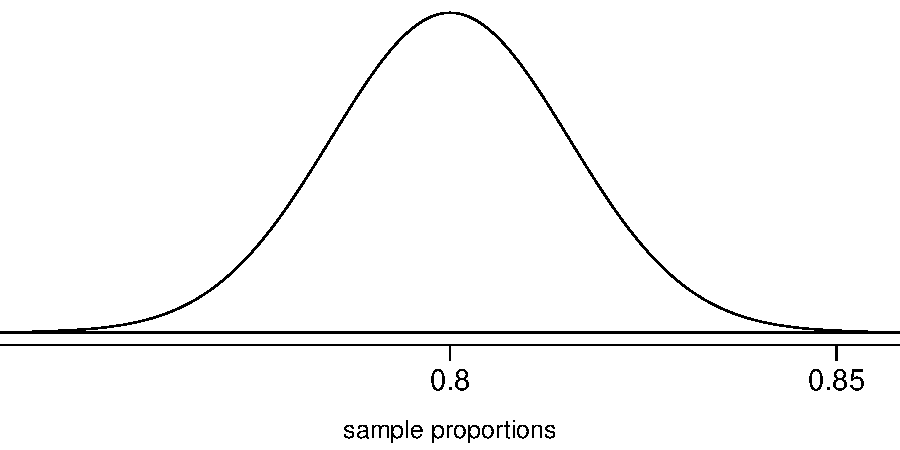
\includegraphics[width=\textwidth]{6-1_single_prop/expdesgn_norm.pdf}
\end{center}
}
\end{frame}
%%%%%%%%%%%%%%%%%%%%%%%%%%%%%%%%%%%

\begin{frame}
\frametitle{Prática}

\justifying
Como o o-valor é baixo, rejeitamos $H_0$. Os dados fornecem evidências convincentes de que mais de 80\% dos americanos têm uma boa intuição sobre desenho de experimentos.

\end{frame}

%%%%%%%%%%%%%%%%%%%%%%%%%%%%%%%%%%%

\subsection{Recapitulando}

%%%%%%%%%%%%%%%%%%%%%%%%%%%%%%%%%%%

\begin{frame}
\frametitle{Prática}

\pq{Em uma pesquisa do Gallup de 2006, 11\% de 1.001 americanos afirmaram que possuem resistência para celebrar o Halloween por motivos religiosos. Ao nível de confiança de 95\%, a margem de erro dessa pesquisa é de $\pm 3\%$. \\
Uma notícia, ao descobrir o resultado dessa pesquisa, publicou: "Mais de 10\% de todos os americanos possuem resistência para celebrar o Halloween por motivos religiosos". \\ Ao nível de confiança de 95\%, a declaração feita nessa notícia é justificada?}

\begin{enumerate}[(a)]
\item Sim
\solnMult{Não}
\item Nao sabe
\end{enumerate}

\end{frame}

%%%%%%%%%%%%%%%%%%%%%%%%%%%%%%%%%%

\begin{frame}
\frametitle{Recapitulando - inferência para uma proporção}

\begin{itemize}

\item Parâmetro da população: $p$, estimativa pontual: $\hat{p}$

\pause

\item Condições:
\begin{itemize}
\item independência \\
- amostra aleatória e condição 10\%
\item pelo menos 10 sucessos e fracassos\\ - se não $\rightarrow$ aleatorizar
\end{itemize}

\pause

\item Desvio Padrão: $SE = \sqrt{ \frac{p(1-p)}{n} }$
\begin{itemize}
\item para IC: usar $\hat{p}$
\item para TH: usar $p_0$
\end{itemize}

\end{itemize}

\end{frame}

